\documentclass[tikz]{standalone}
\begin{document}
\begin{tikzpicture}
	\node[thick,blue,circle,draw] (B) at (2,0)
	{
		\begin{tikzpicture}
			\node[thick,fill,circle] (e) at (0:1) {};
			\node[thick,fill,circle] (g) at (120:1) {};
			\node[thick,fill,circle] (g2) at (240:1) {};
			\draw[->,thick] (e) to[bend right=30] (g);
			\draw[->,thick] (g) to[bend right=30] (g2);
			\draw[->,thick] (g2) to[bend right=30] (e);
			\draw[white] (180:1) circle (0.1);
		\end{tikzpicture}
	};
	\node[thick,blue,circle,draw] (A) at (-2,0)
	{
		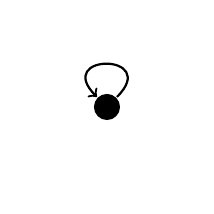
\begin{tikzpicture}
			\node[thick,fill,circle] (e) at (0,0) {};
			\draw[white] (0,0) circle (1);
			\draw[->,thick] (e) to[loop] (e);
		\end{tikzpicture}
	};
	\node[thick,red,circle,draw] (Z) at (4,5)
	{
		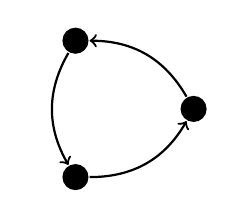
\begin{tikzpicture}
			\node[thick,fill,circle] (e) at (0:1) {};
			\node[thick,fill,circle] (g) at (120:1) {};
			\node[thick,fill,circle] (g2) at (240:1) {};
			\draw[->,thick] (e) to[bend right=30] (g);
			\draw[->,thick] (g) to[bend right=30] (g2);
			\draw[->,thick] (g2) to[bend right=30] (e);
			\draw[white] (180:1) circle (0.1);
		\end{tikzpicture}
	};
	\node[thick,red,circle,draw] (Y) at (0,5)
	{
		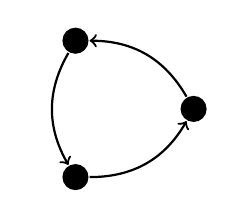
\begin{tikzpicture}
			\node[thick,fill,circle] (e) at (0:1) {};
			\node[thick,fill,circle] (g) at (120:1) {};
			\node[thick,fill,circle] (g2) at (240:1) {};
			\draw[->,thick] (e) to[bend right=30] (g);
			\draw[->,thick] (g) to[bend right=30] (g2);
			\draw[->,thick] (g2) to[bend right=30] (e);
			\draw[white] (180:1) circle (0.1);
		\end{tikzpicture}
	};
	\node[thick,red,circle,draw] (X) at (-4,5)
	{
		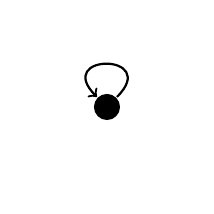
\begin{tikzpicture}
			\node[thick,fill,circle] (e) at (0,0) {};
			\draw[white] (0,0) circle (1);
			\draw[->,thick] (e) to[loop] (e);
		\end{tikzpicture}
	};
	\draw[ultra thick,|->,shorten >=5,shorten <=5] (X) -- (A);
	\draw[ultra thick,|->,shorten >=5,shorten <=5] (Y) -- (A);
	\draw[ultra thick,|->,shorten >=5,shorten <=5] (Z) -- (B);
\end{tikzpicture}
\end{document}
